% !TeX root = ..\rapport_13_2.tex
\section{Design mønstre}
Der har været fokus på at adskille præsentationslag, businesslag, og persistence-lag og flere design mønstre er anvendt for at opnå et let læseligt, overskueligt og lavt koblet system. 

\subsection{Program-lag}
Et klassediagram herunder i \ref{fig:class_persistency} viser relationer mellem klasserne i TaskFusion programmet. TaskFusion fungere som hovedklasse og er primært ansvarlig for brugergodkendelser. Et facade mønster (eng: Facade pattern) er implementeret med \texttt{EmployeeFacade.java} og \texttt{ProjectFacade.java} for at opnå lav kobling. F.eks. bliver systemet, der behandler employees, tilgået gennem \texttt{EmployeeFacade.java} således at klasserne, bestående af bl.a. \texttt{EmployeeRepository.java}, \texttt{Employee.java}, \texttt{RegularActivity.java}, ikke skal kaldes af klienten på forskellig vis. I stedet kan klienten tilgå alle de nødvendige egenskaber igennem facaden kun. Sammen med \textit{EmployeeFacade} og \textit{ProjectFacade} eksponere \textit{TaskFusion} de offentlige metoder der skal kunne tilgås i programmet. På den måde kan vi frihed til at ændre alle metoder i de resterende program-lag, uden det vil påvirke eventuelle brugergrænseflader. Alle metoder i \textit{facade} klasserne kan i virkeligheden ligge i TaskFusion klassen, men ved at opdele metoderne i passende seperate klasser, kan vi bedre vedligeholde og udbygge programmet. 
Programmets domæne lag består af instantierbare objektklasser og er ansvarlig for \textit{Business-logic}. Persistency-laget indeholder \textit{Repositories}, der er ansvarlige for kommunikation med en lagringsløsning. Selvom programmet ikke har et database lag på nuværende tidspunkt, vil det være let at bygge flere lagringsløsninger på senere, ved kun at skulle modificere persistency klasserne. 

\begin{figure}[H]
    \centering
    \caption{Klassediagram over program-laget}
    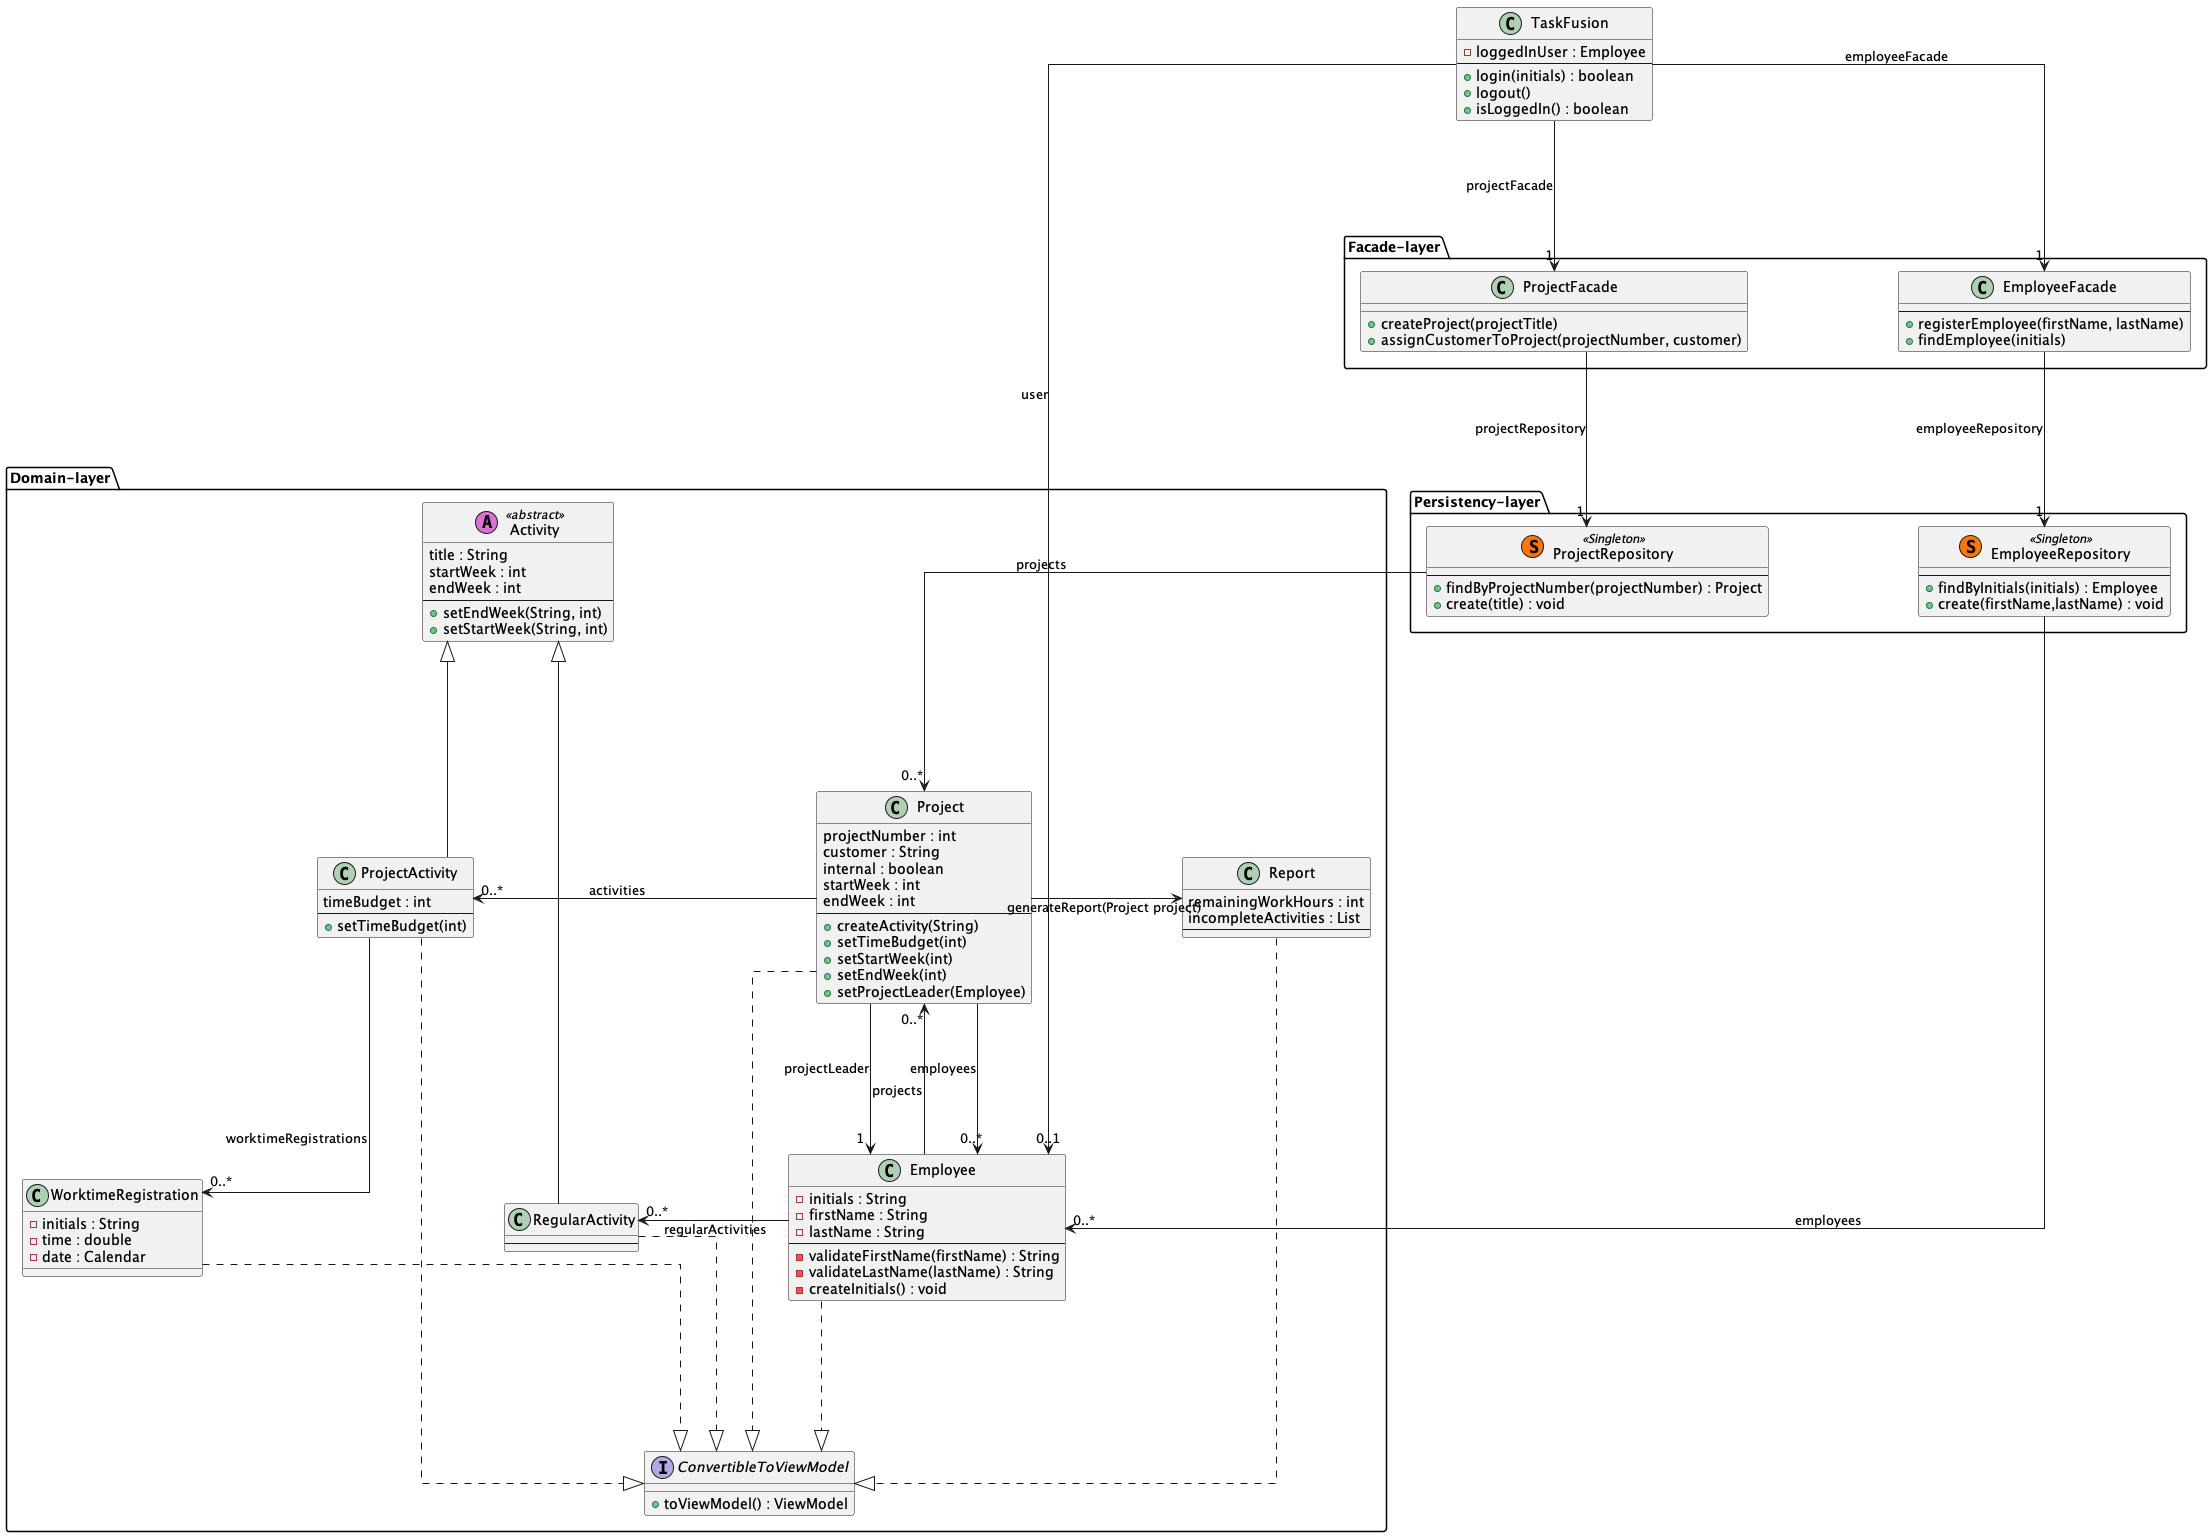
\includegraphics[width = \textwidth, keepaspectratio]{TaskFusion/out/assets/diagrams/class_persistency/ClassDiagram.png}
    \label{fig:class_persistency}
\end{figure}

Vi ønsker desuden aldrig at eksponere programmets klasser udenfor program-laget. Derfor implementere alle instantierbare klasser \textit{ConvertibleToViewModel}-interfacet. Dette interface kræver at klasserne kan eksporteres til en tilsvarende visningsklasse til brug i præsentations-lag. 

Et andet design mønster der er taget i brug, er singleton design mønstret. F.eks. haves et opbevaringssted for alle medarbejdere kaldet \textit{EmployeeRepository}. Der ønskes kun én instans af dette objekt, da idéen er at tilgå og opbevare medarbejderne via. ét objekt. Hvis flere instanser af dette objekt skulle forekomme, er det ikke sikret, at brugeren kan tilgå alle medarbejderne fra den ene instans, da medarbejdere kan eksistere i de andre instanser, hvorfor objektet skal være en singleton. Af samme grunde som EmployeeRepository er en singleton, er ProjectRepository ligeså.
\newline



\subsection{Præsentations-laget}
\noindent Som det blev nævnt i indledningen af dette kapitel, har der været fokus på adskillelse af de forskellige lag i arkitekturen af programmet. Måden hvorpå business-logikken er blevet separeret fra præsentationslaget i programmet er ved brug af Model-View-Controller design mønstret. Dette er gjort ved at have ’controller’ klasser og ’view’ klasser, som har funktionen at modtage forespørgsler fra brugeren og fremvise det efterspurgte data uden at have noget business logik i sig. Disse kan ses under mapperne \textit{controllers} og \textit{views}.

\subsubsection{CLI klassediagram}
\textit{TaskFusionCLI} er hovedklassen når TaskFusion programmet skal benyttes igennem en CLI brugergrænseflade. Når grænsefladen skal interagere med TaskFusion programmet, foregår al kommunikation imellem \textit{Facade}-laget. CLI'en er fundamentalt opbygget med tanke på genbrugelighed, og simplicitet. Det er opnået ved at tage udgangspunkt i en \textit{MenuController}, hvorfra \textit{View}'s bruges til at skrive information brugeren efterspørger til konsollen. Hvordan et \textit{View} ser ud for brugeren, afhænger af hvilke variabler og objekter der gives ved konstruktion af \textit{View}'et. \textit{Component}-klasser er en form for hjælpe klasser, der igennem \texttt{public static} metoder, tilbyder universelle komponenter til brug i grænsefladen.

\begin{figure}[H]
    \centering
    \caption{Klassediagram over præsentations-laget}
    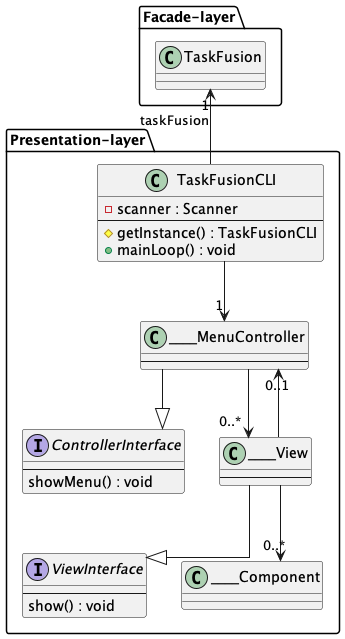
\includegraphics[width = 10cm, keepaspectratio]{TaskFusion/out/assets/diagrams/class_cli/TaskFusion-CLI.png}
    \label{fig:class_cli}
\end{figure}

\subsubsection{CLI brugergrænsefladen}
Da CLI grænsefladen til TaskFusion er opbygget af \textit{MenuController}'re og \textit{View}'s, ender vi da også med et netværk af mulige veje brugeren kan gå. For at få et overblik over TaskFusion, er herunder i \ref{fig:flow_cli} et \textit{flow}-diagram over menuer og sider i CLI grænsefladen.  
\begin{figure}[H]
    \centering
    \caption{Flowdiagram over CLI brugergrænsefladen}
    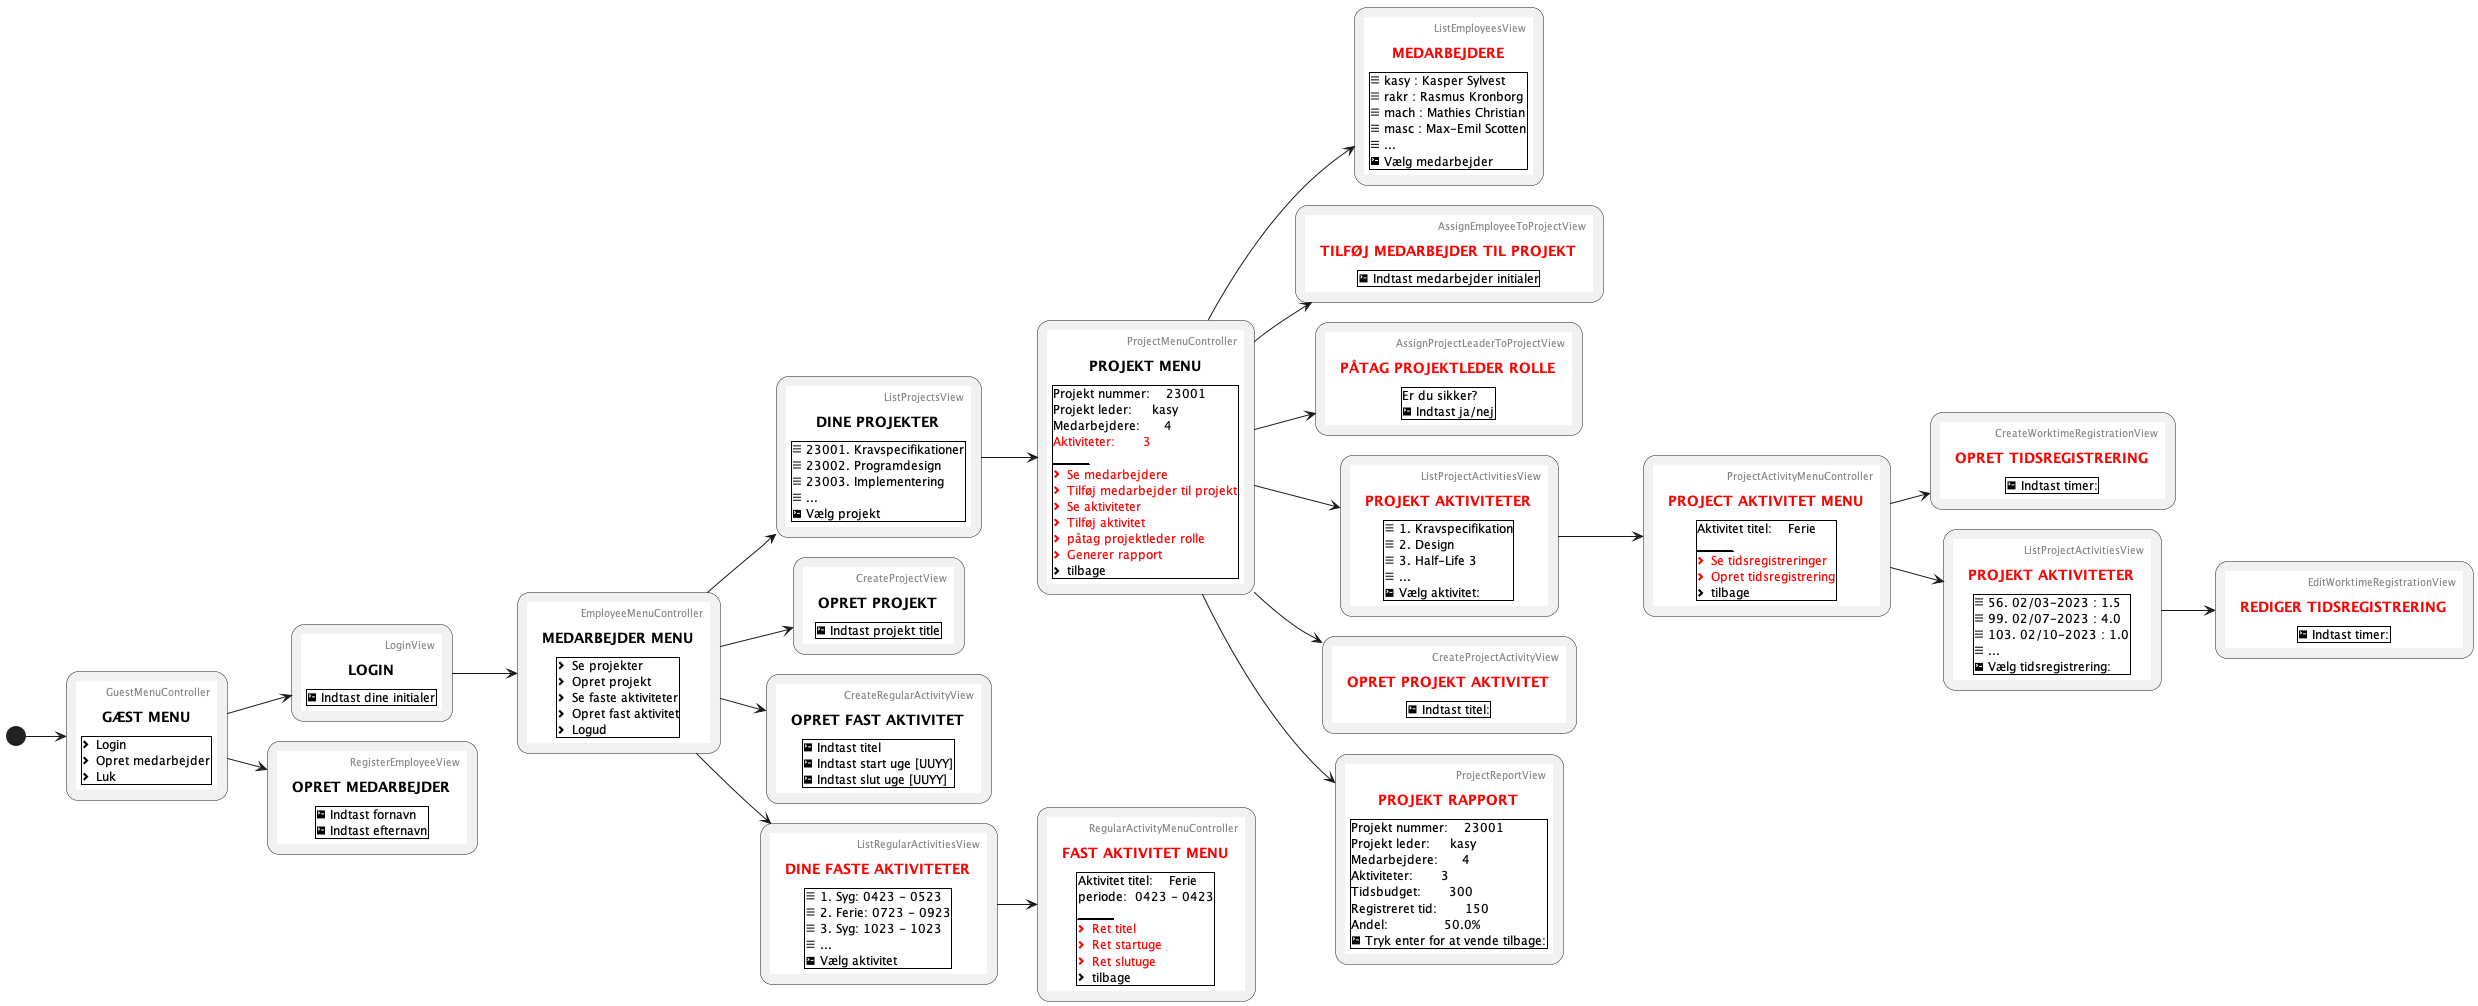
\includegraphics[width = \textwidth, keepaspectratio]{TaskFusion/out/assets/diagrams/flow_cli/flow_cli.png}
    \label{fig:flow_cli}
\end{figure}



\section{SOLID principer}
Nogle SOLID principper er blevet benyttet og vil herunder blive gennemgået med kodeeksempler.

\subsection{Single responsibility principle}
I forbindelse med at designe programmet efter mønstre som nævnt i forrige kapitel, har det også været naturligt at opdele klasser til kun af have et enkelt formål. Det ses som eksempel på \textit{Persistency} klasserne \texttt{ProjectRepository.java} og \texttt{EmployeeRepository}, der henholdsvis har ansvaret for at håndtere de primære hovedobjekt-klasser; \textit{Employee's} og \textit{Project}'s.

Derudover er alle klassers metoder som udgangspunkt lavet til at kun at have et enkelt formål. Herunder i \ref{lst:single_responsibility_source} er to eksempler på metoder fra \texttt{Employee.java}, hvis eneste formål er at validere det givne argument.
\begin{listing}[H]
    \centering
    \caption{Single resposibility metoder}\label{lst:single_responsibility_source}
    \begin{minted}[breaklines]{java}
  private String validateFirstName(String firstName) throws InvalidPropertyException {
    if (firstName.length() < 2) {
      throw new InvalidPropertyException("Fornavn mangler");
    }
    return firstName;
  }

  private String validateLastName(String lastName) throws InvalidPropertyException {
    if (lastName.length() < 2) {
      throw new InvalidPropertyException("Efternavn mangler");
    }
    return lastName;
  }

    \end{minted}
\end{listing}


Der er dog enkelte metoder, der kunne optimeres i forhold til \textit{Single resposibility} principet. Her kan nævnes \textit{createProjectActivity()} som beskrevet i \textit{White box test} kapitlet. Denne metode er både ansvarlig for at acceptere om en medarbejder kan oprette en projekt aktiviet, og derefter også at oprette den. Her kunne man refaktorere til, at tjekket om medarbejderen må oprette en aktivitet, lå udenfor metoden.

\subsection{Open/closed principle}
Det lyder fra opgaveformuleringen, at der skal være mulighed for at opdele projekter op i aktiviteter, og at der skal være mulighed for at lave faste aktiviteter til registrering af bl.a. ferie og kurser, som ikke er knyttet til projekter. Et simpelt eksempel hvor open-closed princippet er blevet benyttet til at imødekomme førnævnte er at lave en abstrakt klasse kaldet \texttt{activity.java}, som vist herunder i figur \ref{fig:class_open_closed_example}. Denne har de enkelte felter som \texttt{title}, \texttt{startweek}, \texttt{endweek}, samt exceptions og getter-metoder og ikke mere. Det er muligt at udvide (extend) denne klasse således at der kan laves to underklasser, \texttt{ProjectActivity.java} og \texttt{RegularActivity.java}. På den måde er \texttt{Activity} lukket for ændringer men åben for udvidelser. 
\begin{figure}[H]
    \centering
    \caption{Klassediagram af \textit{aktivity} klasserne}
    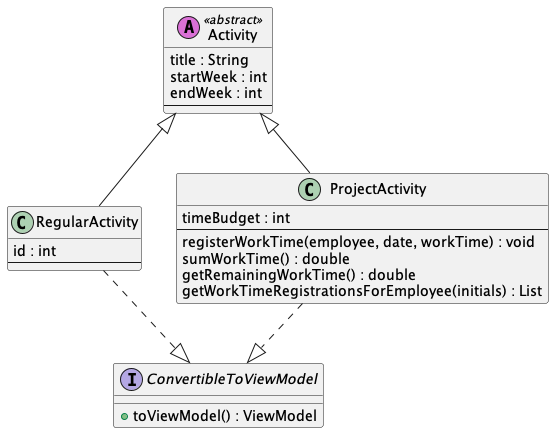
\includegraphics[width = 15cm, keepaspectratio]{TaskFusion/out/assets/diagrams/class_open_closed_example/class_open_closed_example.png}
    \label{fig:class_open_closed_example}
\end{figure}

Der er desuden også det argument, at \textit{single responsibilty princippet} bliver fulgt, da \texttt{Activity.java} klassen kun har én grund til at blive ændret. Den grund vil indbefatte en ændring af definitionen, af hvad en aktivitet er, f.eks. en ændring af dets felter.


\subsection{Liskov substitution principle}



\subsection{Interface segregation principle}



\subsection{Dependency inverseion principle}

